\subsection{Warning of transformer loss spikes}\label{sec:spike-warning}
As a transformer learns modular addition, its loss can spike abruptly. We compare warning rules on development runs, maximizing the number of spikes warned of subject to at most two false alarms per 10,000 scored updates. The selected rule checks every 50 updates and warns when MG of the latest 500 log losses is at or below 6.3144 (rounded). A spike counts as detected if at least one warning occurs in the 500 updates before its onset. This rule warned of 22 of 23 evaluation spikes, including the one in Figure~\ref{fig:slingshot-warning} with 195 updates to spare. Roughness, the standard deviation of successive log-loss differences divided by that of the log losses, warned of all 23 at the same evaluation false-alarm rate (Table~\ref{tab:spikes_campaign}).

\begin{figure*}[!htb]
\centering
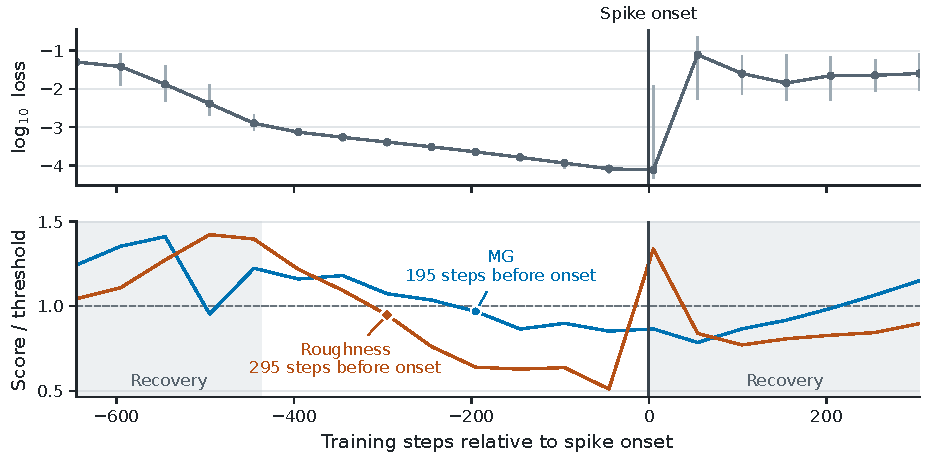
\includegraphics[width=.92\textwidth]{figures/slingshot_warning.pdf}
\caption{A loss spike in an evaluation run. The top band shows the minimum and maximum log loss around the mean in each block. Blue shading marks the interval for successful warnings. Dotted lines show the thresholds chosen on development runs. Dots mark the first warnings.}
\label{fig:slingshot-warning}
\end{figure*}

\Needspace{7\baselineskip}
\subsection[Model selection from scalar logs]{Model selection from scalar logs}\label{sec:ssl}
We train image encoders on different views of each MNIST digit without using its label. To score an encoder, we freeze it and train a linear digit classifier on its features. On two development repeats we choose the scalar log and ranking direction with the highest mean Spearman correlation with classifier accuracy. The resulting rule picks the encoder with the highest MG over its final 1,000 gradient norms. Across five new repeats its choice averages 0.41 percentage points below the best of 29 configurations. A statistic using features from many images ranks the full set slightly better (Figure~\ref{fig:ssl-probe-scatter} and Table~\ref{tab:ssl_campaign}).
